\documentclass[11pt,a4paper,final,notitlepage]{report}
\usepackage[utf8]{inputenc}
\usepackage{amsmath}
\usepackage{amsfonts}
\usepackage{amssymb}
\usepackage{fullpage}
\usepackage{graphicx}
\usepackage{url}
\renewcommand{\baselinestretch}{1.25} %Increase 

\makeatletter
\newcommand*{\toccontents}{\@starttoc{toc}}
\makeatother

\newcommand{\noNumberChapter}[2]{
    \setcounter{chapter}{#1}
    \setcounter{section}{0}
    \chapter*{#2}
    \addcontentsline{toc}{chapter}{#2}
}

\begin{document}

\title{Specialist Production Module\\
	   Renderman Ice Shader}

\author{Tom Minor - Level I\\
		Software Development for Animation, Games and Effects\\
		Bournemouth University - NCCA}

\maketitle

\renewcommand{\abstractname}{Project Overview}
\begin{abstract}
%% 			What's my focus area? (CG Ice Cubes)
\begin{center}
In this project I aimed to develop a \textit{physically based \textbf{Ice Cube Shader}} in \textit{Renderman Shading Language}.
\end{center}

\end{abstract}


\toccontents

%% Talk about :

%%			Why I chose shaders (wanted to learn them properly)
%%			Why I chose ice cube (wanted to do ice, but decided to pace myself and focus on just an ice cube, allowed me to collect primary research much easier than travelling to real life ice caves)
%%			Why Renderman (industry standard, fast, learning shaders once gives me a transferrable skill, offline rendering relieves me of the worry of having to make them behave well in real-time etc
\noNumberChapter{0}{Introduction}

\begin{center}
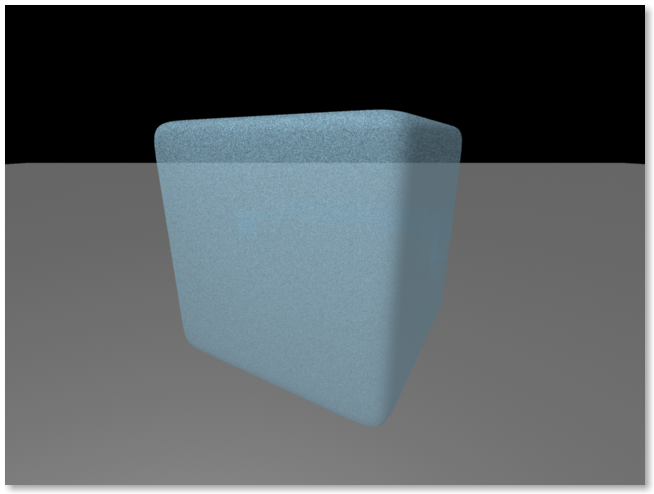
\includegraphics[scale=0.65]{../../../Pictures/testscene.png} 
\end{center}


Todo

\noNumberChapter{1}{Initial Research}
\section{Primary - Experiments with real ice cube and light}


\section{Secondary - Relevant papers}


\section{Reading the documentation and tutorials}
%% Tutor suggested I look into superquads (insert picture)


The Renderman documentation was invaluable for understanding the
\cite{Nishino:2012:VSF:2407746.2407747}

\noNumberChapter{2}{Production}
\section{Initial Tests}
\section{Results}
\section{Unforeseen Problems}

\noNumberChapter{3}{Conclusion}

\nocite{*}

\bibliographystyle{plain-annote}
\bibliography{bib_icereport}
\end{document}